
% ----------------------------------------------------------------------
\subsection{Simulación de señales}

% C- Módulo de generación de medidas asociadas a una trayectoria
% - Objetivo del módulo		
En este módulo se podrán simular distintos tipos de señales a partir de la trayectoria generada por el módulo anterior. El objetivo es generar los datos que los algoritmo de posicionamiento procesarán. Al igual que en el módulo anterior, los modelos de simulación son cruciales para que el comportamiento del simulador sea fiel a la realidad. 
% - Modelización	
%     - Tipos de señales y métricas			
En navindoor se han definido dos tipo de señales, unas que dependen de la posición de balizas y otras que solo dependen de la trayectoria; eston son objetos \emph{BeaconBased} y \emph{BeaconFree} respectivamente (figura \ref{schemaBB}). Es clasificación es debido a que los parámetros de entrada para la generación de estas señales son distintos.

%     - Diagrama de clases
\begin{figure}[ht!]
    \centering
        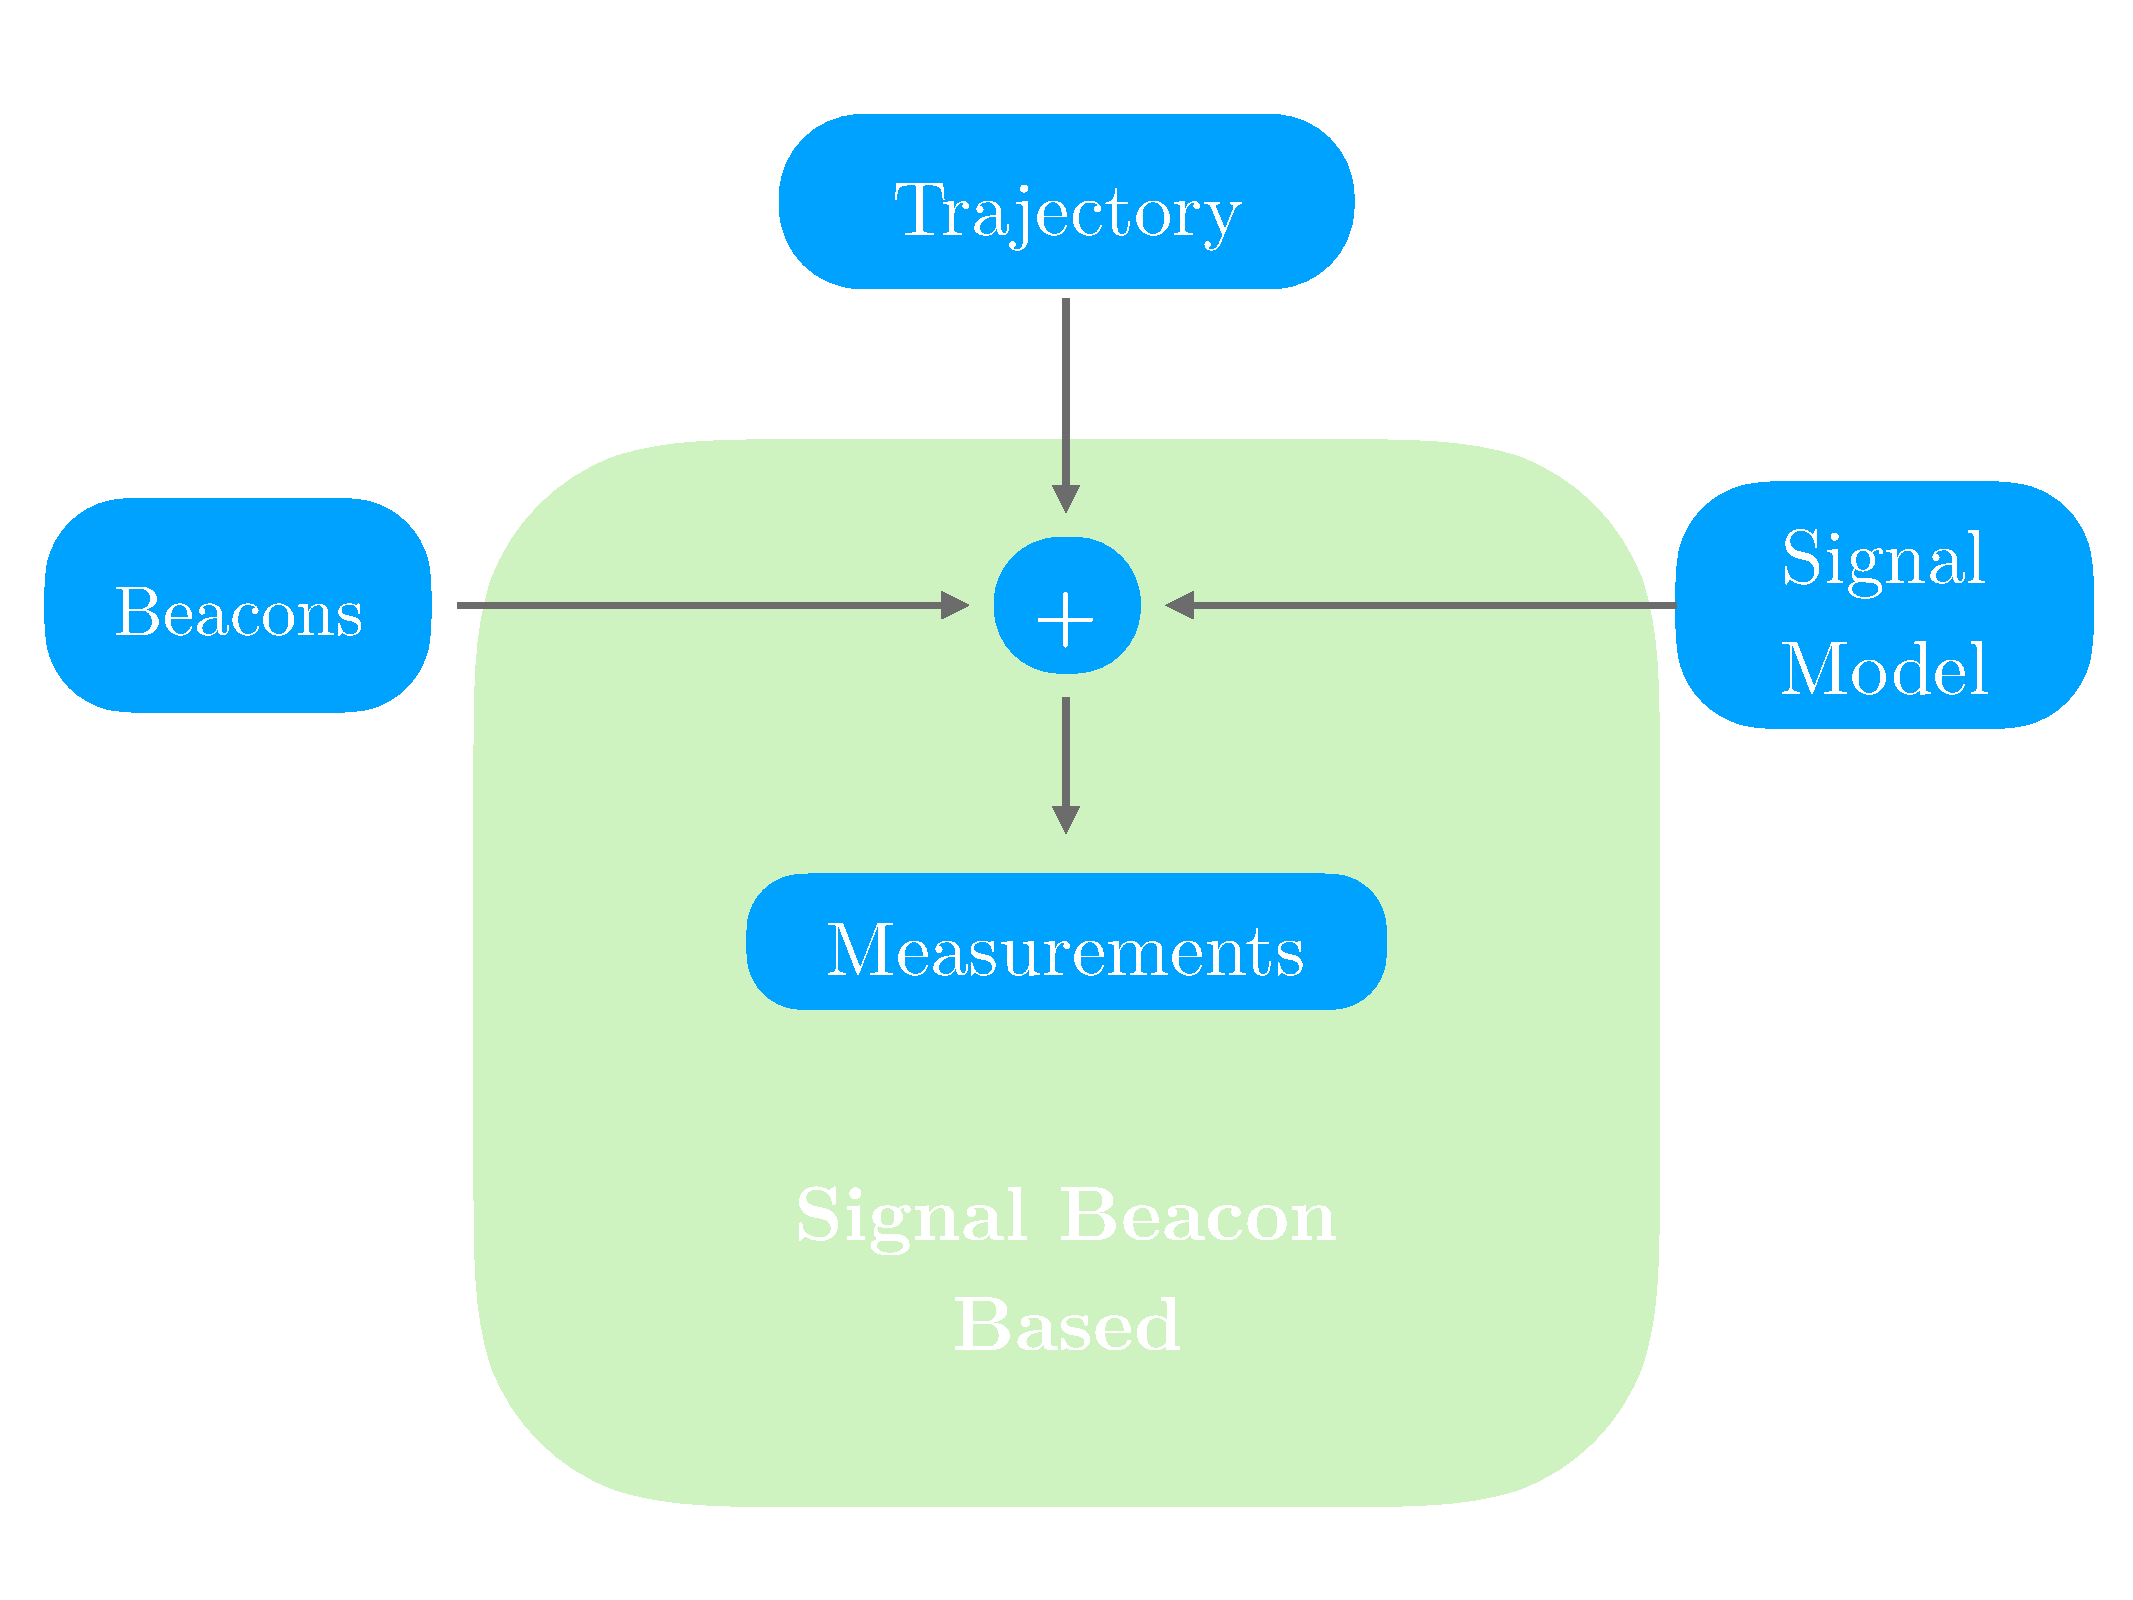
\includegraphics[width=0.8\columnwidth]{img/Design/4.pdf}
        \caption{Representación de la construcción de las señales.}
        \footnotesize
        Se muestra un esquema de la construcción de las señales. Estas necesitan la trayectoria y un modelo de simulación. En el caso de la señales \emph{BeaconBased}, además necestian los objetos \emph{beacons} de definidos en el modulo de planimetría.
        \label{schemaBB}
    \end{figure}


% - Explicación básica del proceso de generación de medidas asociada a una trayectoria: 
%     - Modelos de ruido: parámetros, crear modelos nuevos
%     - Visualizar señal generada













La simulación de señales se realiza a partir del objeto de la trayectoria. La trayectoria más un modelo de generación de señales son lo mínimo necesario para crear los objetos señales. En navindoor se han definido dos tipo de señales, unas que dependen de la posición de balizas y otras que solo dependen de la trayectoria; eston son objetos \emph{BeaconBased} y \emph{BeaconFree} respectivamente (figura \ref{schemaBB}). 

\begin{figure}
    \centering
        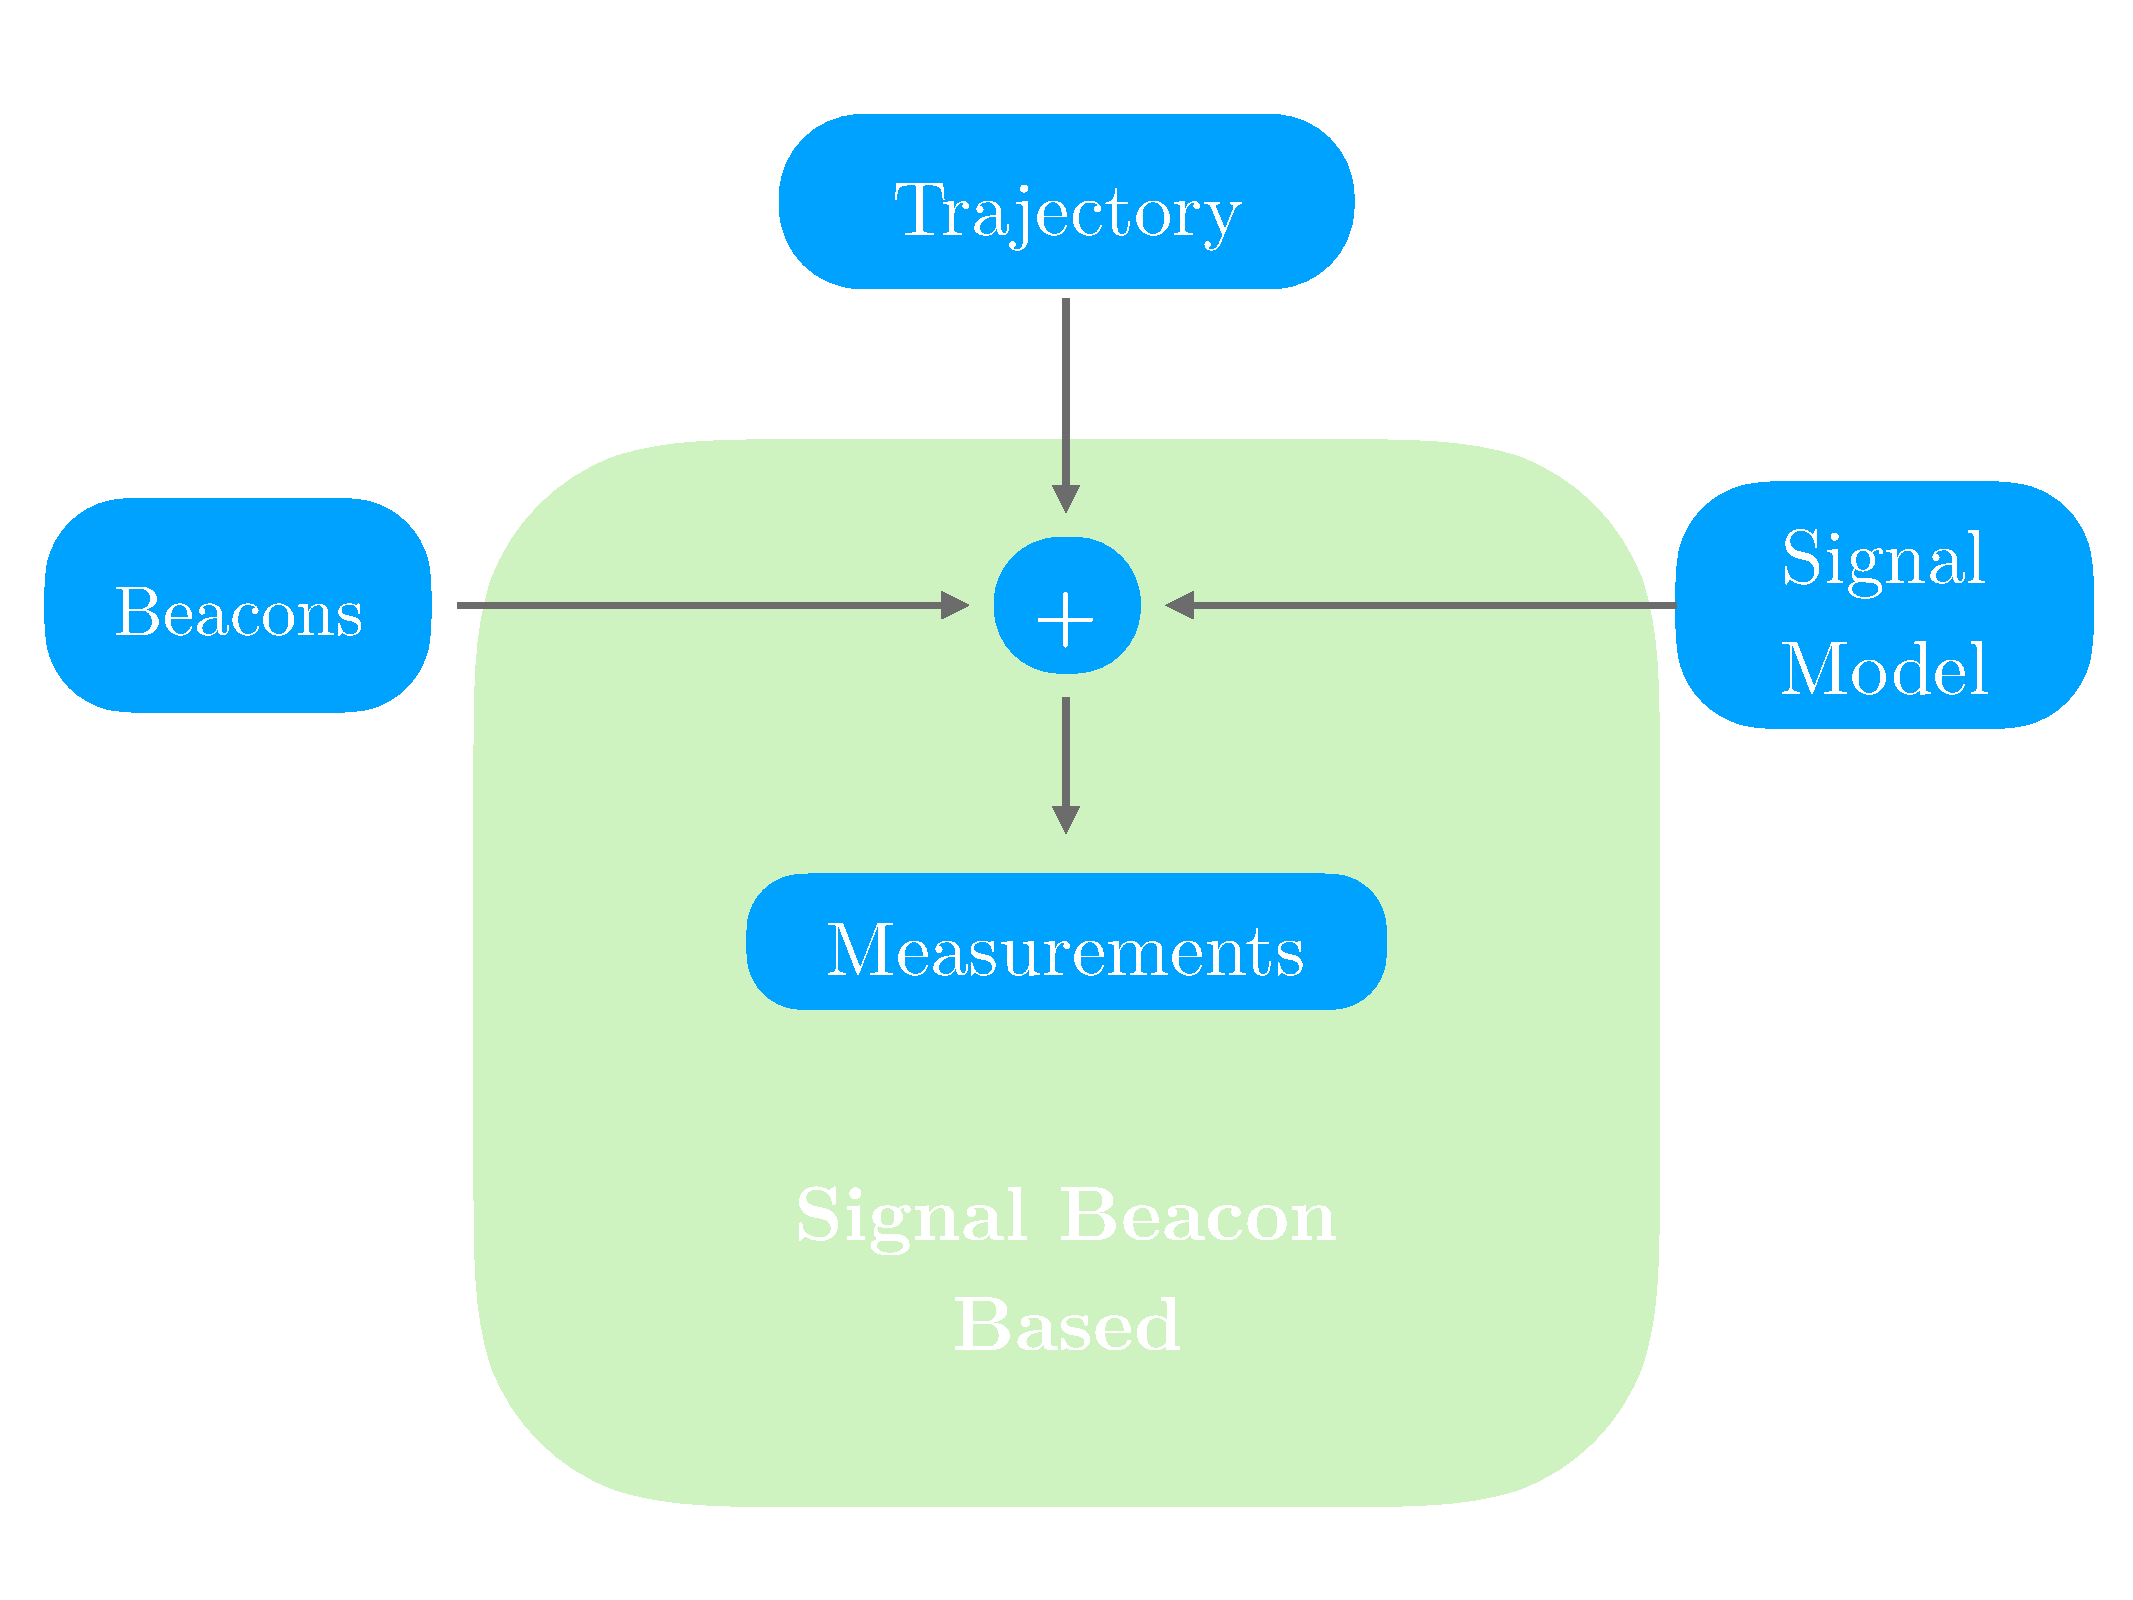
\includegraphics[width=0.8\columnwidth]{img/Design/4.pdf}
        \caption{Representación de la construcción de las señales.}
        \footnotesize
        Se muestra un esquema de la construcción de las señales. Estas necesitan la trayectoria y un modelo de simulación. En el caso de la señales \emph{BeaconBased}, además necestian los objetos \emph{beacons} de definidos en el modulo de planimetría.
        \label{schemaBB}
    \end{figure}


\begin{table}[ht]
    \centering
    \begin{tabular}{|c|c|}
        \hline
        {\textbf{BeaconBased}} & {\textbf{BeaconFree}}          \\ \hline
        {Received Signal Strength (RSS)}    & Barómetro        \\ \hline
        {Time of flight (ToF)}              & Acelerómetro               \\ \hline
        {Angle of Arrival (AoA)}            & Magnetómetro             \\ \hline
    \end{tabular}
    \caption{Tipo de modelos de simulación de señales}
    \label{tiposenales}
\end{table}

Al igual que en los modelos de simulación de trayectorias. Los modelos de generación de señales no son más que parámetros de entrada del constructor de las señales. Dentro de los tipo de modelos que pueden implementarse en navindoor se pueden ver en la tabla \ref{tiposenales}. Se ha implementado un modelo para cada tipo de señales. 




\begin{figure}[!ht]
    \centering
    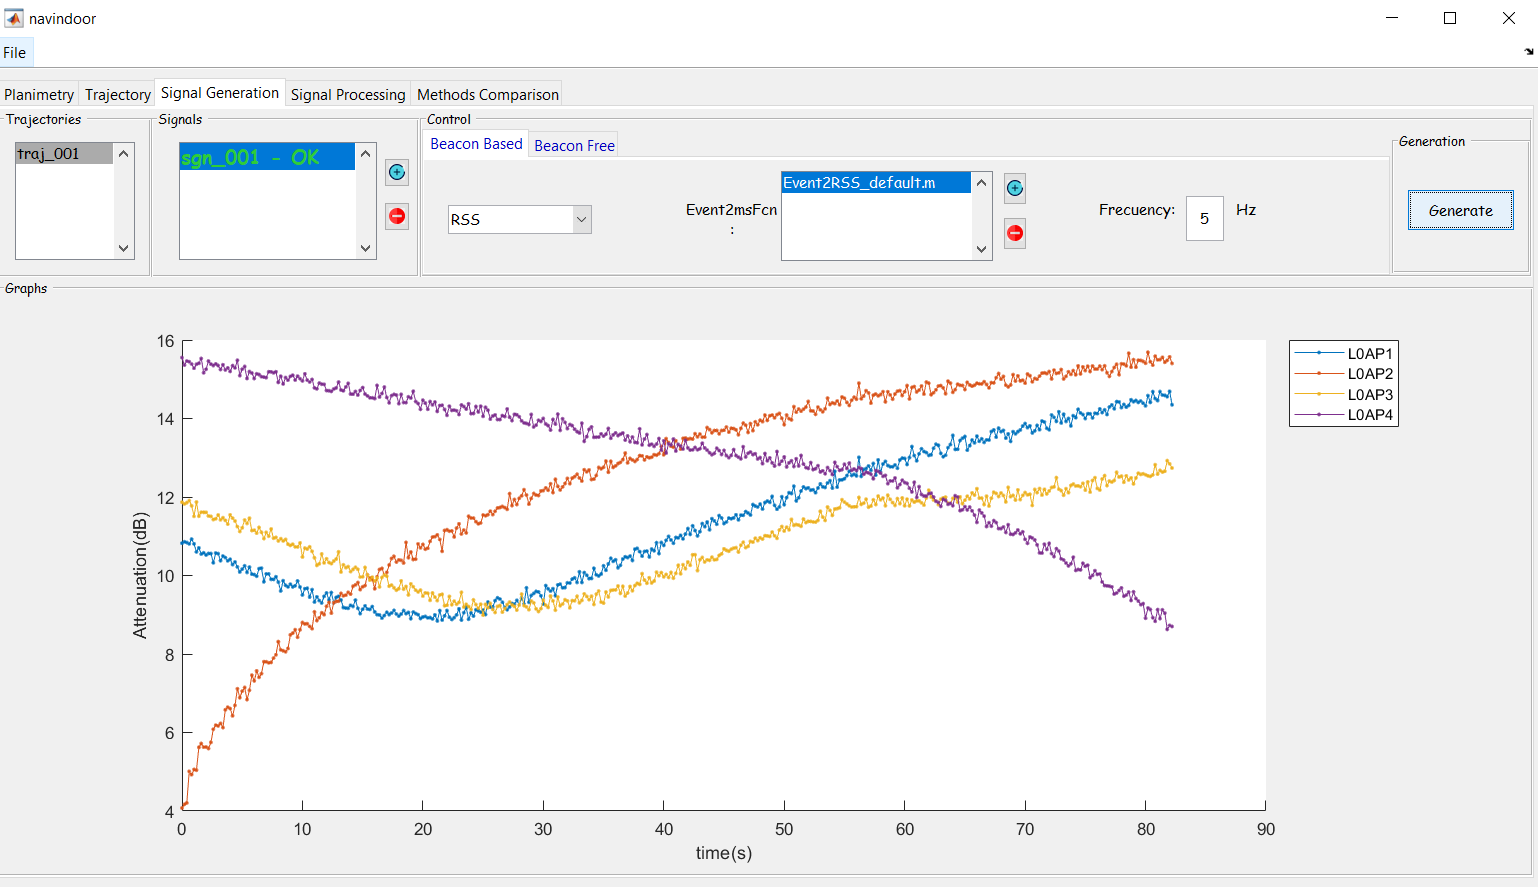
\includegraphics[width=0.8\columnwidth]{img/Design/3.PNG}
    \caption[]{Interfaz gráfica para el módulo de las señales}
    \footnotesize
    En esta captura se puede ver la representación de una señales RSS, en una planimetría con cuarto \emph{beacons}. La gráfica la evolución en el tiempo de la atenuación de cada uno de los \emph{beacons}
    \label{fig:interfaz3}
\end{figure}


